\documentclass[xcolor=dvipsnames]{beamer}
%\documentclass[usenames,dvipsnames]{beamer}
\usepackage[utf8]{inputenc}
\usepackage[T1]{fontenc}
\usepackage{tikz}
\usepackage{xytree}
\usepackage{comment}
\usepackage{multirow}
\usepackage{cancel}
\usepackage{colortbl}
\usepackage{tikz-qtree}
\usepackage{comment}

\usepackage{graphicx}
\usepackage{array}
%\usepackage{avm}
\usepackage{rotating}
\usepackage{amssymb}
\usepackage{makecell}
%\usepackage[british]{babel}
%\usepackage[utf8x,utf8]{inputenc}
\usepackage{xcolor}
\usepackage{enumitem}
\usepackage{eurosym}
\usepackage{hyperref}
\usepackage{comment}

\usepackage{xcolor}

%\newcommand{\ile}[1] {{\scriptsize \textcolor{RoyalBlue}{\textit{#1}}}}
%\newcommand{\lit}[1]{{\scriptsize \textcolor{RoyalBlue}{`#1'}}} %Literal translation
%\newcommand{\idio}[1]{{\scriptsize \textcolor{RoyalBlue}{`#1'}}}  %Idiomatic translation
%\newcommand{\exlit}[2]{\ile{#1}~\lit{#2}} %Example with a literal translation
%\newcommand{\exidio}[2]{\ile{#1}~\idio{#2}} %Example with an idiomatic translation
%\newcommand{\litidio}[2]{\lit{#1}$~\Rightarrow~$\idio{#2}} %Literal and idiomatic translation
%\newcommand{\exlitidio}[3]{\ile{#1}~\lit{#2}~$\Rightarrow$~\idio{#3}} %Example with a literal and a and idiomatic translation

\newcommand{\ana}[1] {{\scriptsize \textcolor{RoyalBlue}{#1}}} %Output of an analysis of a text 
\newcommand{\iletrue}[1] {\textcolor{OliveGreen}{#1}}
\newcommand{\ilefalse}[1] {\textcolor{Red}{#1}}
\newcommand{\ileunsure}[1] {\textcolor{BurntOrange}{#1}}
%\newcommand{\lex}[1] {\textbf{#1}} %Lexicalized component


%%%%%%%%%%%
%% in-line examples for languages in Latin script
%%%%%%%%%%
\usepackage{ulem}
\newcommand{\lex}[1]{\textbf{#1}}  %Lexicalized component
\newcommand{\litlex}[1]{\uwave{#1}}  %Literal reading of a lexicalized component
\newcommand{\coinlex}[1]{\dashuline{#1}}  %Coincindental co-occurrence of lexicalized components

\newcommand{\ile}[1]{\textcolor{blue}{\textsl{#1}}} %In-line example  
\newcommand{\lit}[1]{\textcolor{gray}{(lit. '\textit{#1}')}} %Literal translation
\newcommand{\idio}[1]{\textcolor{brown}{`#1'}}  %Idiomatic translation
\newcommand{\exlit}[2]{\ile{#1}~\lit{#2}} %Example with a literal translation
\newcommand{\exidio}[2]{\ile{#1}~\idio{#2}} %Example with an idiomatic translation
\newcommand{\litidio}[2]{\lit{#1}~\idio{#2}} %Literal and idiomatic translation
\newcommand{\exlitidio}[3]{\ile{#1}~\lit{#2}~\idio{#3}} %Example with a literal and a and idiomatic translation


%%%%%%%%%%
\setbeamertemplate{itemize/enumerate subbody begin}{\scriptsize}

\usepackage{relsize}
\newcommand{\lang}[1]{\textcolor{gray}{\textsmaller[1.5]{\fbox{\textsf{#1}}}}}

\newcommand{\formatPOS}[1]{{\scriptsize #1}}
\newcommand{\formatMorph}[1]{\_}  %{{\tiny #1}}
\newcommand{\formatMWE}[1]{\textcolor{blue}{#1}}

\newcommand*\GBitem{%
   \item[{
\includegraphics[width=0.2cm]{Images/Flags/UnitedKingdom.png}}]}
\newcommand*\FRitem{%
   \item[{
\includegraphics[width=0.2cm]{Images/Flags/France.png}}]}
\newcommand*\PLitem{%
   \item[{\includegraphics[width=0.2cm]{Images/Flags/Poland.png}}]}
\newcommand*\SRitem{%
   \item[{\includegraphics[width=0.2cm]{Images/Flags/Serbia.png}}]}
\newcommand*\ITitem{%
   \item[{\includegraphics[width=0.2cm]{Images/Flags/Italy.png}}]}

\newcommand{\gloss}[1] {
  {\scriptsize \textcolor{blue}{'#1'}}}

%%%%% Linguistic examples in blue scriptsize italic
\newcommand{\exa}[1]{\textcolor{blue}{\textit{#1}}}

%%%%% Bibliographic references in scriptsize
\newcommand{\mycite}[1]{{\scriptsize \textcolor{magenta}{\cite{#1}}}}
\newcommand{\minicite}[1]{{\scriptsize \cite{#1}}}
%\newcommand{\minicitet}[1]{{\scriptsize \citet{#1}}}

%%%%% Bets results
\newcommand{\best}[1]{\textbf{#1}}



\usetheme{Darmstadt}
\setbeamertemplate{footline}
{
  \leavevmode%
  \hbox{%
  \begin{beamercolorbox}[wd=.333333\paperwidth,ht=2.25ex,dp=1ex,center]{author in head/foot}%
    \usebeamerfont{author in head/foot}\insertshortauthor%~~\beamer@ifempty{\insertshortinstitute}{}{(\insertshortinstitute)}
  \end{beamercolorbox}%
  \begin{beamercolorbox}[wd=.333333\paperwidth,ht=2.25ex,dp=1ex,center]{title in head/foot}%
    \usebeamerfont{title in head/foot}\insertshorttitle
  \end{beamercolorbox}%
  \begin{beamercolorbox}[wd=.333333\paperwidth,ht=2.25ex,dp=1ex,right]{date in head/foot}%
    \usebeamerfont{date in head/foot}\insertshortdate{}
    \hspace*{2em}
    \insertframenumber{} / \inserttotalframenumber\hspace*{2ex} 
  \end{beamercolorbox}}%
  \vskip0pt%
}
\setbeamertemplate{navigation symbols}{}
\beamertemplatenavigationsymbolsempty


%\usecolortheme[RGB={0,100,100}]{structure}
%\usecolortheme[named=BrickRed]{structure}

\setbeamerfont{author}{size=\large}
\setbeamerfont{title}{series=\bfseries,size=\LARGE}
%%%%%%%%%%%%%%%%%%%%%%%%%%%%%%%%%%%%%%%%%%%%%%%%%%%%%%%%%%%%%%%%%%%%%%%%
%\usecolortheme{crane}
\usecolortheme{seagull}

\setlist{labelindent=1em,leftmargin=1em}
\setitemize{label=\usebeamerfont*{itemize item}%
  \usebeamercolor[fg]{itemize item}
  \usebeamertemplate{itemize item}}




%%%%%%%%%%%%%%%%%%%%%%%%%%%%%%%%%%%%%%%%%%%%%%%%%%%%%%%%%%%%%%%%%%%%%%%%%%%%%%%%%%%%

\title[PARSEME Intro]{Introduction to annotating verbal multiword expressions in the PARSEME framework\\
\includegraphics[scale=0.3]{Images/parseme-logo.png}}

\author{Carlos Ramisch, Agata Savary}

\institute[shortinst]{Aix-Marseille Université, Université Paris-Saclay, France}



\date[UniDive, 19/06/2023]{UniDive webinar, 19 June 2023}

\begin{document}

%\frame{\titlepage}
\begin{frame}

\titlepage
%\textgreek{καλημέρα & καλωσήρθατε στην}
\end{frame}

%%%%%%%%%%%%%%%%%%%%%%%%%%%%%%%%%%%%%%%%%%%%
\section{PARSEME} 
\subsection{}

%%%%%%%%%%%%%
\begin{frame}
  \frametitle{PARSEME}
  
\begin{scriptsize}
  
\begin{block}{Network}
\begin{itemize}
\item COST Action on \textbf{Parsing and Multiword Expressions} (MWEs) funded by European Commission in \textbf{2013-2017}, still \textbf{active}
\item 31 countries, 30 languages and 6 dialects from 10 language genera
\item Outcomes: publications, resources, tutorials, methodologies, PMWE book series 
\end{itemize}
\end{block}

\begin{block}{MWE corpora (\textcolor{magenta}{\url{https://gitlab.com/parseme/corpora/-/wikis/}})}
\begin{itemize}
\item \textbf{Collaborative} effort: 25 language teams, 31 language leaders, 160 annotators
\item Annotation \textbf{guidelines} for \textbf{verbal} MWEs \textbf{unified} across some 25 languages
\item Corpora \textbf{manually} annotated for MWEs: \textbf{25 languages}, open licenses
\item \textbf{Continuous enhancements} of the guidelines and corpora
\end{itemize}
\end{block}

\end{scriptsize}

\begin{tikzpicture}[remember picture,overlay]
\node at (8.5,6.8) {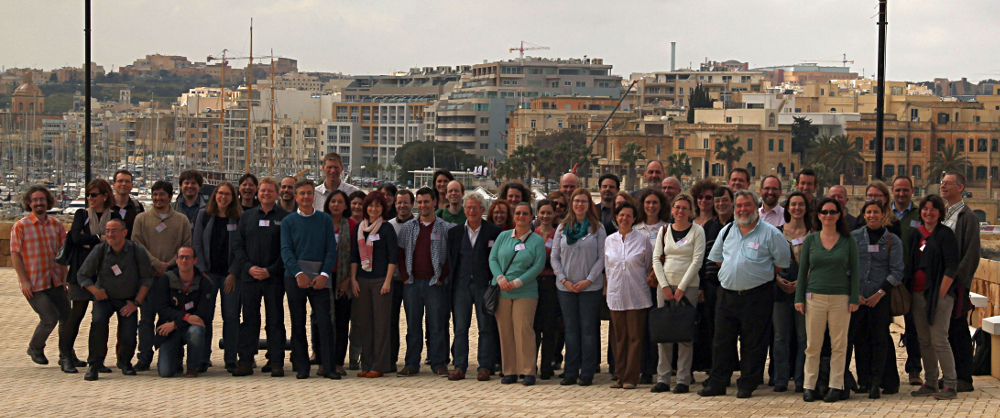
\includegraphics[scale=0.15]{Images/parseme-malta.jpg}};
\end{tikzpicture}

\end{frame}


%%%%%%%%%%%%%%%%%%%%%%%%%%%%%%%%%%%%%%%%%%%
\section{MWEs} 
\subsection{}

%%%%%%%%%%%%%
\begin{frame}
  \frametitle{Multiword expressions}

\begin{block}{}
\textit{The \textcolor{red}{\textbf{prime time}} speech by \textcolor{blue}{\textbf{first lady}} \textcolor{green}{\textbf{Michelle Obama}} \textcolor{magenta}{\textbf{set}} the house \textcolor{magenta}{\textbf{on fire}}. She made \textcolor{brown}{\textbf{crystal clear}} which issues she \textcolor{violet}{\textbf{took to heart}} but she was \textcolor{orange}{\textbf{preaching to the choir}}.}
\end{block}

\begin{block}{Definition \cite{baldwin-kim:2010:handbook}}
Combination of at least \textbf{two words} which exhibits lexical, morphological, syntactic, semantic and /or statistical \textbf{idiosyncrasies}.
\end{block}

\begin{block}{Idiosyncrasy}
A mode of behaviour or a property which is \textbf{particular} to an (few) individual(s). An \textbf{unusual} feature.
\end{block}


\end{frame}

%%%%%%%%%%%%%

\begin{frame}
  \frametitle{MWE's \exidio{X-factor}{special quality}}

%\begin{scriptsize}

\begin{block}{Non-compositional semantics}
   \begin{itemize}
   \item The meaning of a MWE is surprising, given the meanings of its component words
      \begin{itemize}
      \item[]\lang{EN} \exidio{to \lex{pull} one's \lex{leg}}{to tease someone playfully}
      \item[]\lang{IT} \exlitidio{\lex{lasciar perdere}}{to let lose}{to give up}
      \end{itemize}
   \end{itemize}
\end{block}

\begin{block}{Challenge}
Semantic non-compositionality is \textbf{hard to test directly}.
\end{block}

%\end{scriptsize}

\end{frame}


%%%%%%%%%%%%%%%
\begin{frame} 
\frametitle{Inflexibility: a proxy for semantic non-compositionality}

\begin{block}{Hypothesis}
A MWE is \textbf{less flexible} than a regular construction of the same syntactic structure.
\end{block}

\vspace{0.5cm}

\begin{scriptsize}
\centering
\setlength{\tabcolsep}{0.5mm}
\begin{tabular}{|l|p{5.4cm}|p{1.8cm}|}\hline
\textbf{Regular construction} & \textbf{MWE} & \begin{tabular}{l}\textbf{MWE}\\\textbf{property}\end{tabular} \\\hline\hline

  \begin{tabular}{l}\ile{warm soup} $\approx$\footnote{{\tiny '$\approx$' means that the meaning shift is predictable from the formal change}} \ile{hot soup} $\approx$ \\ \ile{warm stew}\end{tabular}
& \begin{tabular}{l}\ile{\lex{hot dog}} vs. \ile{\#warm dog} vs. \ile{\#hot terrier}\end{tabular}
& \begin{tabular}{l}Lexical\\inflexibility\end{tabular} \\\hline

  \begin{tabular}{l}\ile{to throw meat to the lions} $\approx$ \\ \ile{to throw meat to the \underline{lion}}\end{tabular}
& \begin{tabular}{l}\ile{to \lex{throw} someone \lex{to the lions}} vs. \\ \ile{\#to throw someone to the \underline{lion}}\end{tabular}
& \begin{tabular}{l}Morphological\\inflexibility\end{tabular} \\\hline

  \begin{tabular}{l}\ile{the die is stolen} $\approx$ \\ \ile{\underline{someone stole} the die}\end{tabular}
& \begin{tabular}{l}\ile{\lex{the die is cast}} vs. \\ \ile{\#\underline{someone cast} the die}\end{tabular} 
& \begin{tabular}{l}Syntactic\\inflexibility\end{tabular} \\\hline

\end{tabular}
\end{scriptsize}

\end{frame}

%%%%%%%%%%%%%%%%
\begin{frame} 
\frametitle{Focus on \textbf{verbal} MWEs -- challenges}

\begin{scriptsize}
\begin{itemize}
\item Discontinuity:
	\begin{itemize}
	\item[] \lang{EN} \ile{Trying hard to \textbf{bear} all these more or less important indications \textbf{in mind}}
	\item[] \lang{DE} \ile{Klaus Kinkel (FDP) \textbf{ging} in seiner Würdigung des Mauerfalls zumindest auf den 9. November 1938 \textbf{ein}.}
    	\end{itemize}
\item Flexibility: morphological, syntactic, lexical
	\begin{itemize}
	\item[] \lang{EN} \ile{he \lex{broke} my \lex{fall}} vs.~\ile{both of my \lex{falls} were hard to \lex{break}}
	\end{itemize}
\item Ambiguity: idiomatic vs.~literal readings
	\begin{itemize}
	\item[] \lang{EN} \exidio{she \lex{takes the cake}}{she is the most outstanding} vs. \ile{she takes the cake}
	\end{itemize}
\item Overlaps:
   	\begin{itemize}
	\item[] \lang{EN} \ile{\underline{\lex{take}} a \lex{walk} and then a long \lex{shower}} (coordination)
	\item[] \lang{EN} \ile{\lex{take} the fact that I \underline{\lex{gave up}} \lex{into account}} (interleaving)
	\item[] \lang{EN} \ile{\lex{\underline{let} the cat \underline{out} of the bag}} (nesting)
	\end{itemize}
\item Multiword tokens
	\begin{itemize}
	\item[] \lang{ES}  \exlitidio{\lex{abstener}|\lex{se}}{abstain oneself}{abstain} vs. \ile{me abstengo}
	\item[] \lang{DE}  \exlitidio{\lex{auf}|\lex{machen}}{out|make}{open} vs. \ile{macht auf}
	\end{itemize}
\item Different languages $\Rightarrow$ different behavior, linguistic traditions\ldots
\end{itemize}
\end{scriptsize}

\end{frame}

%%%%%%%%%%%%%%%%
\begin{frame} 
\frametitle{Neutralizing flexibility}

\begin{block}{Canonical form}
Least syntactically marked syntactic variant which preserves the idiomatic reading (active voice is less marked then passive, etc.)

\begin{tabular}{ccc}
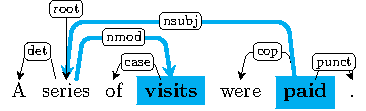
\includegraphics[width=.45\textwidth]{Images/series-of-visits-paid} & 
$\Longrightarrow$ &
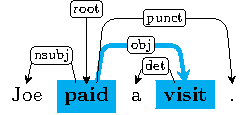
\includegraphics[width=.25\textwidth]{Images/pay-visit}
\end{tabular}

\end{block}

\begin{block}{}
Canonical forms are useful for \textbf{formalizing} the morpho-syntactic properties of MWEs. This is useful e.g. for \textbf{annotation guidelines}.
\end{block}

\end{frame}

%%%%%%%%%%%%%%%%%%%%%%%%%%%%%%%%%%%%%%%%%%%
\section{Annotation} 
\subsection{}

%%%%%%%%%%%%%%%%
\begin{frame} 
\frametitle{Annotating MWEs in a corpus}

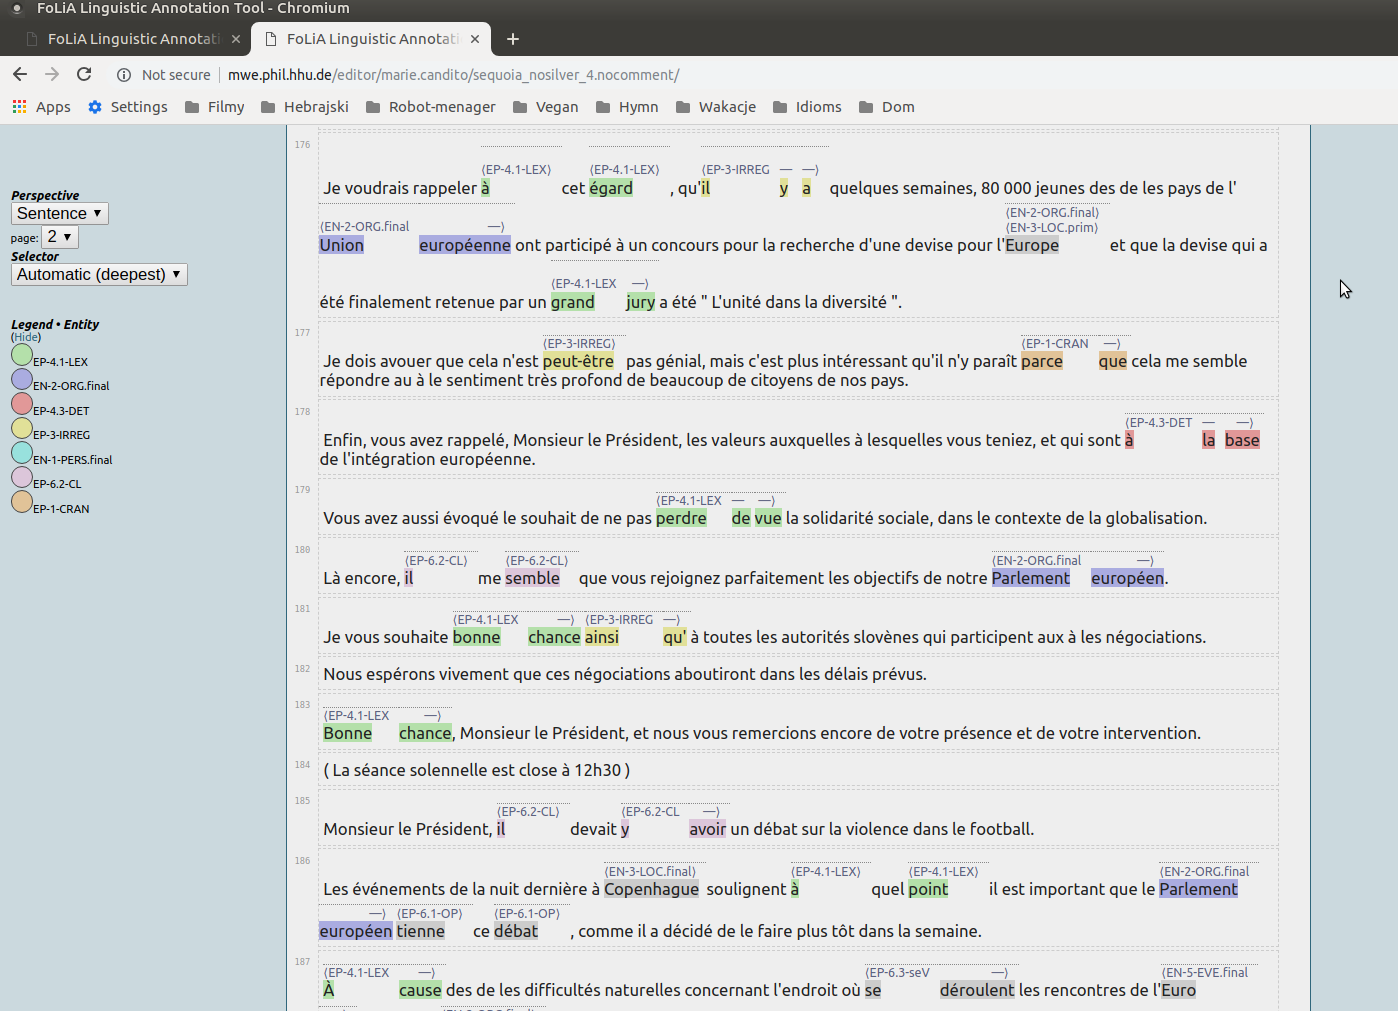
\includegraphics[scale=0.23]{Images/flat.png}

\end{frame}

%%%%%%%%%%%%%
\begin{frame}
  \frametitle{PARSEME annotation guidelines \textcolor{magenta}{{\scriptsize (\url{https://parsemefr.lis-lab.fr/parseme-st-guidelines/1.2})}}}

%\begin{scriptsize}

\vspace{-0.2cm}

\begin{block}{Objectives} 
\begin{itemize}
\item Formalise idiomaticity in a \textbf{cross-linguistically unified} and \textbf{computationally tractable} way
\item Unify what is truly \textbf{similar}, emphasise what is \textbf{language-specific}
\item Make the annotation \textbf{reproducible}
\end{itemize}
\end{block}

%\end{scriptsize}

\end{frame}


%%%%%%%%%%%%%%%%%%%%%%%
\begin{frame}
  \vspace*{-5pt}
  \frametitle{VMWE typology (v. 1.2)}

\begin{scriptsize}
\begin{block}{}
\begin{itemize}
\item \textbf{Universal} categories (valid for all languages):
   \begin{itemize}
   \item light verb constructions (\textbf{LVCs})
	\begin{itemize}
	\item \textbf{LVC.full}: \lang{EN} \ile{to \lex{give} a \lex{lecture}}
	\item \textbf{LVC.cause}: \lang{EN} \ile{to \lex{grant} \lex{rights}}
	\end{itemize}
   \item verbal idioms (\textbf{VIDs})
	\begin{itemize}
	\item[] \lang{EN} \ile{to \lex{call it a day}}
	\end{itemize}
   \end{itemize}
\item \textbf{Quasi-universal} categories (valid for many languages):
   \begin{itemize}
   \item inherently reflexive verbs (\textbf{IRVs})
	\begin{itemize}
	\item[] \lang{FR} \exidio{\textcolor{RoyalBlue}{\lex{s'évanouir}}}{to faint}
	\end{itemize}
   \item verb-particle constructions (\textbf{VPCs})
	\begin{itemize}
	\item \textbf{VPC.full} \lang{EN} \exidio{to \lex{do in}}{to kill}
	\item \textbf{VPC.semi} \lang{EN} \exidio{to \lex{eat up}}{to eat completely}
	\end{itemize}
   \item multi-verb constructions (\textbf{MVCs})
	\begin{itemize}
	\item[] \lang{HI} \exlitidio{\textcolor{BlueViolet}{\lex{kar le-na}}}{do take.INF}{to do something (for one's own benefit)}
	\end{itemize}
   \end{itemize}
\item \textbf{Experimental} (optional) category
   \begin{itemize}
   \item inherently adpositional verbs (\textbf{IAVs})
	\begin{itemize}
	\item[] \lang{EN} \ile{to \lex{come across} sth/sb}, \ile{to \lex{rely on} sth/sb}
	\end{itemize}	
   \end{itemize}
\end{itemize}
\end{block}
\end{scriptsize}

\end{frame}


%%%%%%%%%%%%%%%%
\begin{frame} 
\frametitle{Towards reproducibility -- guidelines as decision diagrams}

\centering
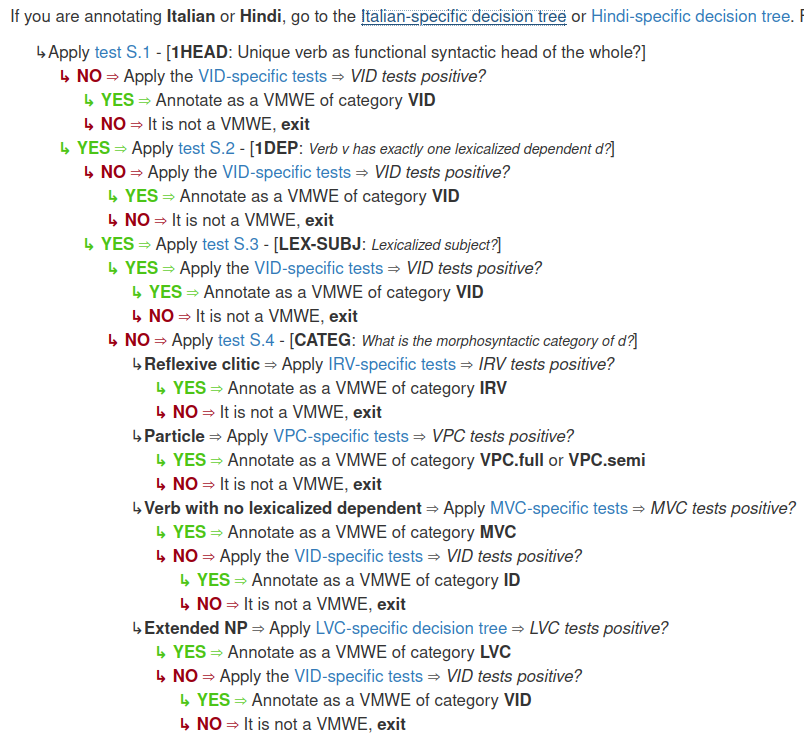
\includegraphics[scale=0.3]{Images/decision-diagram}


\end{frame}


%%%%%%%%%%%%%%%%
\begin{frame} 
\frametitle{Annotation exercise 1 \href{https://mwe.phil.hhu.de/}{\beamergotobutton{[FLAT]}}\href{http://parsemefr.lif.univ-mrs.fr/parseme-st-guidelines/1.3}{\beamergotobutton{[guidelines]}}}

\ile{the fate of the republic rests on your shoulders} (sentence 4)

\begin{scriptsize}
\begin{block}{}
\begin{itemize}
\item Step 1: identify the candidate and its canonical form: \ile{rests on your shoulders}
\item Step 2: determine the lexicalized components
   \begin{itemize}
   \item \ile{\lex{rests on} your/our \lex{shoulders}}, \ile{\lex{rests on} the \lex{shoulders} of the deputies}, etc.
   \end{itemize}
\item Follow the \href{http://parsemefr.lif.univ-mrs.fr/parseme-st-guidelines/1.3/?page=040\_Annotation\_process\_-\_decision\_tree}{\beamergotobutton{decision tree}}
   \begin{itemize}
   \item S.1 [1HEAD] (YES): \ile{rests} is the only verbal head of the whole phrase
   \item S.2 [1DEP] (YES): \ile{on shoulders} is the only lexicalized dependent of \ile{rests}
   \item S.3 [LEX-SUBJ] (NO): \ile{on} shoulders is not the subject of \ile{rests}
   \item S.4 [CATEG] (extended NP): \ile{on shoulders} is a prepositional phrase
   \item LVC.0 [N-ABS] (NO): \ile{shoulders} is not abstract
   \item VID.1 [CRAN] (NO): all components function also as stand-alone words
   \item VID.2 [LEX] (YES): \#\ile{remains on your shoulders}, \#\ile{rests on your back/arms/head}
   \end{itemize}
\item Outcome: \textbf{VID}
\end{itemize}
\end{block}

\end{scriptsize}

\end{frame}


%%%%%%%%%%%%%%%%
\begin{frame} 
\frametitle{Annotation exercise 2}

\ile{I hate to put a little pressure on you} (sentence 4)

\begin{scriptsize}
\begin{block}{}
\begin{itemize}
\item Step 1: identify the candidate and its canonical form: \ile{put a little pressure on you}
\item Step 2: determine the lexicalized components
   \begin{itemize}
   \item \ile{\lex{put} a little \lex{pressure} on you}, \ile{\underline{put} more/no/a lot of \underline{pressure}}, etc.
   \end{itemize}
\item Follow the \href{http://parsemefr.lif.univ-mrs.fr/parseme-st-guidelines/1.3/?page=040\_Annotation\_process\_-\_decision\_tree}{\beamergotobutton{decision tree}}
   \begin{itemize}
   \item S.1 (YES) $\rightarrow$ S.2 (YES) $\rightarrow$ S.3 (NO) $\rightarrow$ S.4 (extended NP) $\rightarrow$
   \item LVC.0 [N-ABS] (YES): \ile{pressure} is not abstract
   \item LVC.1 [N-PRED] (YES): 2 semantic arguments: (i) the person putting pressure, (ii) the person subject to the pressure
   \item LVC.2 [V-SUBJ-N-ARG] (YES): I is the subject of \ile{put} and the agent of \ile{pressure} 
   \item LVC.3 [V-LIGHT] (YES): \ile{\lex{put pressure}} $\approx$ force
   \item LVC.4 [V-REDUC] (YES): \ile{my pressure on you}
   \end{itemize}
\item Outcome: \textbf{LVC.full}
\end{itemize}
\end{block}

\end{scriptsize}

\end{frame}

%%%%%%%%%%%%%%%%%
\begin{frame} 
\frametitle{Annotation exercise 3}

\ile{Mr Osborne signed up with a US speakers agency} (sentence 26)

\begin{scriptsize}
\begin{block}{}
\begin{itemize}
\item Steps 1-2: identify the candidate and its canonical form: \ile{\underline{sign up}} or \ile{\underline{sign up with}}
   \begin{itemize}
   \item A VMWE in its proptotypical form is a verbal phrase in active voice whose head verb is in a finite for and whose \underline{other lexicalized components depend either on the verb or on another lexicalized component}
   \item In the the lexical (as opposed to functional) approach to dependency grammar \underline{prepositions depend on the nouns} they introduce $\Rightarrow$ \ile{\underline{sign up}}
   \end{itemize}
\item Follow the \href{http://parsemefr.lif.univ-mrs.fr/parseme-st-guidelines/1.3/?page=040\_Annotation\_process\_-\_decision\_tree}{\beamergotobutton{decision tree}}
   \begin{itemize}
   \item S.1 (YES) $\rightarrow$ S.2 (YES) $\rightarrow$ S.3 (NO) $\rightarrow$ PREP.EN.1 (YES) $\rightarrow$ S.4 (particle) $\rightarrow$
   \item VPC.1 [PART-REDUC] (YES): \exidio{sign up}{to sign one's name (as to a contract) in order to join something} and \ile{sign} refer to the same event
   \item VPC.2 [PART-SPATIAL] (NO): \ile{up} is not spatial in the context of \ile{sign}
   \item VPC.3 [PART-SPATIAL-LIT] (NO): there is no literal reading of \ile{sign up} with \ile{up} being spatial
   \end{itemize}
\item Outcome: \textbf{VPC.semi}
\end{itemize}
\end{block}

\end{scriptsize}

\end{frame}

%%%%%%%%%%%%%%%%%
\begin{frame} 
\frametitle{Annotation exercise 4}

\ile{Opportunity for Beijing to demonstrate its ambitions} (sentence 44)

\begin{scriptsize}
\begin{block}{}
\begin{itemize}
\item Steps 1-2: identify the candidate and its canonical form: \ile{\underline{demonstrate} its \underline{ambitions}} 
\item Follow the \href{http://parsemefr.lif.univ-mrs.fr/parseme-st-guidelines/1.3/?page=040\_Annotation\_process\_-\_decision\_tree}{\beamergotobutton{decision tree}}
   \begin{itemize}
   \item LVC.0 [N-ABS] (YES): \ile{ambition} is abstract
   \item LVC.1 [N-PRED] (YES): 2 semantic arguments: (i) the person/group having the ambition, (ii) object of the ambition
   \item LVC.2 [V-SUBJ-N-ARG] (YES): \ile{Bejing} is the subject of \ile{demonstrate} and the agent of \ile{ambitions}
   \item LVC.3 [V-LIGHT] (NO): \ile{ambitions} can exist without being demonstrated
   \item VID.1, VID. 2, VID.3, VID.4, VID5 (NO): \ile{demonstrate}/\ile{show}/\ile{display} \ile{its} \ile{ambitions}/\ile{aspirations}/\ile{desires}
   \end{itemize}
\item Outcome: \textbf{no VMWE}
\end{itemize}
\end{block}

\end{scriptsize}

\end{frame}


\begin{frame} 
\frametitle{Homework}

Take the text in English and try to annotate the following sentences:

\begin{block}{}
\begin{itemize}
\item \ile{We \underline{face} a lot of \underline{competition}} (sentence 14)
\item \ile{There are \underline{parallels} to \underline{draw}} (sentence 17)
\item \ile{\underline{Vote} was \underline{cast}} (sentence 18)
\item \ile{The date for \underline{cutting the first steel}} (sentence 27)
\item \ile{To \underline{charge} passengers an access \underline{fee}} (sentence 36)
\item \ile{\underline{put} new \underline{limits}} (sentence 54)
\item \ile{\underline{The few ruin it for the many}} (sentence 45)
\item \ile{\underline{Took down} popular websites} (sentence 46)
\item \ile{We are \underline{moving in the right direction}} (sentence 50)
\end{itemize}
\end{block}

\end{frame}

%%%%%%%%%%%%%%%
\begin{frame} 
\frametitle{PARSEME infrastructure}

\begin{block}{}
\begin{itemize}
\item PARSEME wiki - extensive documentation of the corpora and tools  \href{https://gitlab.com/parseme/corpora/-/wikis}{\beamergotobutton{[link]}}
\item Language Leader guide
\item User guides
\item Gitlab repositories for all languages %\href{https://gitlab.com/parseme/corpora/-/wikis/home#languages}{\beamergotobutton{[language table]}}
\item Corpus validators, converters, filters, release automation \ldots
\item Data quality tools
   \begin{itemize}
   \item Consistency checks %\href{https://grew.fr/download/PARSEME/pt.html}{\beamergotobutton{[e.g. for Portuguese]}}
   \end{itemize} 
\item Corpus browser: Grew-match $\longrightarrow$ see the \textbf{tutorial by Bruno} in a few minutes
\end{itemize}
\end{block}

\end{frame}

%%%%%%%%%%%%%%%%%
%%%%%%%%%%%%%%%%%%%%%%%%%%%%%%%%%%%%%%%%%
\section{Wrap-up}  
\subsection{}

%%%%%%%%%%%%%%%%%%%%%%%
\begin{frame}
   \frametitle{PARSEME annotation framework -- conclusions}

\begin{scriptsize}

\begin{block}{Principles and constraints} 
\begin{itemize}
\item The annotations guidelines are \textbf{unified} accross 26 languages with relatively few \textbf{language-specific} sections 
\item Annotation follows a \textbf{decision diagram} (unique starting point), for the sake of \textbf{reproducibility}
\item Non-compositionality is a matter of \textbf{scale} but decisions must be \textbf{binary}
\item \textbf{Semantic non-compositionality} is the major property to capture but is \textbf{hard to test directly}
\item Lexical and morpho-syntactic \textbf{inflexibility} is considered a \textbf{proxy} for semantic non-compositionality
\item Inflexibility tests are driven by the \textbf{syntactic structure}
\item Strong dependence on the underlying \textbf{syntactic theory}
\item PARSEME annotation largely \textbf{relies on the UD} annotation of morpho-syntax
\end{itemize}
\end{block}

\end{scriptsize}

\end{frame}


%%%%%%%%%%%%%%%%%%%%%%%
\setbeamertemplate{footline}{}
\newcounter{finalframe}
\setcounter{finalframe}{\value{framenumber}}
%%%%%%%%%%%%%%%%%%%%%%%

%%%%%%%%%%%%%%%%%%%%%%%%%%%%%%

\setcounter{framenumber}{\value{finalframe}}
%%%%%%%%%%%%%%%%
\section{Bibliography} %and Motivation
\subsection{}
%%%%%%%%%%%%%%%%

\scriptsize{\bibliographystyle{natbib-compact}}
%\scriptsize{\bibliographystyle{plainnat}}

\begin{frame}[allowframebreaks]
\frametitle{Bibliography}

\tiny{\bibliography{biblio}}

\end{frame}

%%%%%%%%%%%%%%%%%%%%%%%%%%%%%%
\setcounter{framenumber}{\value{finalframe}}
%%%%%%%%%%%%%%%%%%%%%%%%%%%%%%


\end{document}

